\documentclass[12pt, letterpaper]{article}

\title{AA279c Project Report: Modeling the ISS}
\author{Toby J. Buckley}
\date{\today}




\usepackage{graphicx}
\usepackage{subcaption}
\usepackage{float}

\graphicspath{{./src/html/}}
\DeclareGraphicsExtensions{.pdf,.png,.jpg}

\begin{document}

\begin{titlepage}
	\maketitle
\end{titlepage}


testing



% 4 thrusters - 13.3 kg-f (29.3 lbf) https://www.quora.com/How-does-the-International-Space-Station-maintain-its-orbit-and-what-propellant-does-it-use



\section{Problem Set 8 - Implement Actuators and Controllers}

\begin{figure}[H]
	\centering
	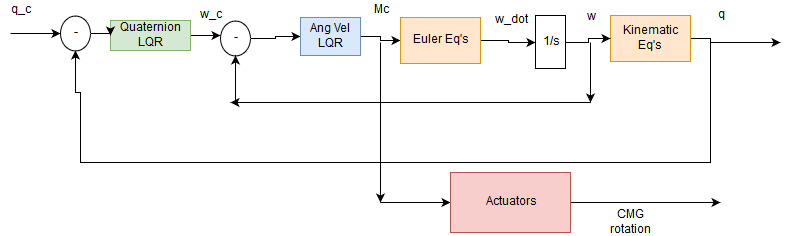
\includegraphics[scale=0.7]{PS8_controller}
	\caption{Block diagram for the controller used onboard the satellite. Two LQR's are utilized, one for attitude and the other for a lower-level ang. vel. controller.}
	\label{8:controller}
\end{figure}


\begin{figure}[H]
	\centering
	\includegraphics[scale=0.9]{ps8_01}
	\caption{Angular velocity while de-tumbling.}
	\label{8:angvel}
\end{figure}


\begin{figure}[H]
	\centering
	\includegraphics[scale=0.9]{ps8_02}
	\caption{Angular velocity while de-tumbling.}
	\label{8:angvel}
\end{figure}


\begin{figure}[H]
	\centering
	\includegraphics[scale=0.9]{ps8_03}
	\caption{Angular velocity while de-tumbling.}
	\label{8:angvel}
\end{figure}


\begin{figure}[H]
	\centering
	\includegraphics[scale=0.9]{ps8_04}
	\caption{Angular velocity while de-tumbling.}
	\label{8:angvel}
\end{figure}


\begin{figure}[H]
	\centering
	\includegraphics[scale=0.9]{ps8_05}
	\caption{Angular velocity while de-tumbling.}
	\label{8:angvel}
\end{figure}





\section{Problem Set 9 - Define and Execute a Slew Maneuver}
A problem all satellites deal with is de-tumbling. When launched into orbit the satellite is harshly ejected from its rocket into a target orbit and must immediately begin to align itself into its nominal position. I've simulated a tumbling environment by setting $w0=rand(3,1)$ and allowing the dynamics and controller to stabilize the system naturally. The target attitude for the de-tumble is the earth-facing RTN frame.


\begin{figure}[H]
	\centering
	\includegraphics[scale=0.9]{ps9_01}
	\caption{Angular velocity while de-tumbling.}
	\label{9:angvel}
\end{figure}

Fig. \ref{9:angvel} shows the angular velocity while de-tumbling. Because of the high priority on matching $w$ to $w_{desired}$ the velocities stabilize quickly. After that all changes are due to the attitude controller commanding certain angular velocity in order to align itself with the RTN frame.


\begin{figure}[H]
	\centering
	\begin{subfigure}[b]{0.49\textwidth}
	\includegraphics[width=\textwidth]{ps9_02}
	\end{subfigure}
	\begin{subfigure}[b]{0.49\textwidth}
		\includegraphics[width=\textwidth]{ps9_03}
	\end{subfigure}
	\caption{The position during a de-tumble. The Target is earth-facing in the RTN frame.}
	\label{(9:pos)}
\end{figure}

Fig. \ref{(9:pos)} shows how the principle axes aligns itself with the RTN frame over time. Oscillations are present due to the sinusoidal dynamics of the rotation cosine matrices.

\begin{figure}[H]
	\centering
	\includegraphics[scale=0.9]{ps9_04}
	\caption{Attitude control error until convergence.}
	\label{9:atterror}
\end{figure}

Fig \ref{9:atterror} shows the evolution of the attitude control error over time. It's clear the the tumbling has a huge effect on the relative alignment of the principle axes with the desired RTN frame. But this problem is overcome within 800 seconds of ejection with the satellite's onboard controller.




\end{document}